\chapter{Result}
\label{chap:Result}

\section{Result}
首先是观察SURF初步匹配的情况。

\begin{center}
    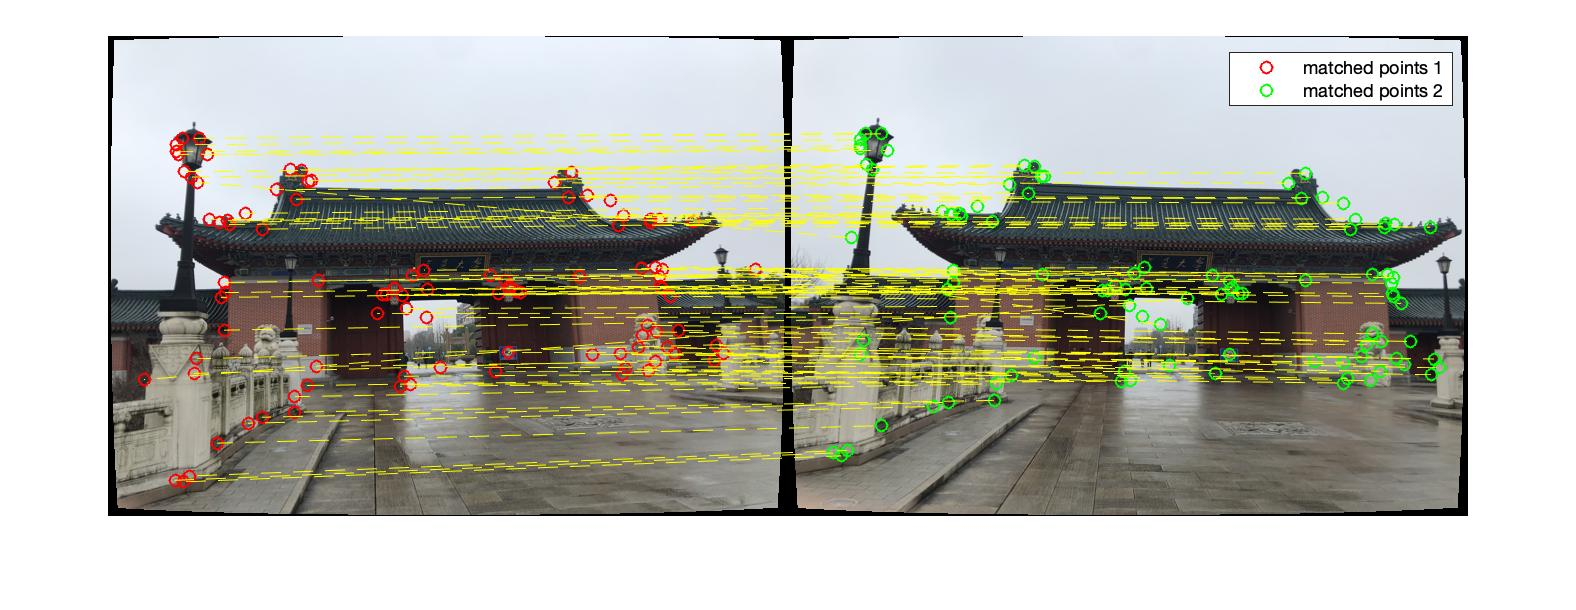
\includegraphics[width=0.9\textwidth]{figures/1.jpg}
\end{center}

我们可以发现图片的边界有一点变化,这是由于做完畸变矫正的原因。其次我们可以看到大部分的对应点都是相互对应的。表现比较好

接下来我们再看一下做完了RANSEC之后的结果。
\begin{center}
    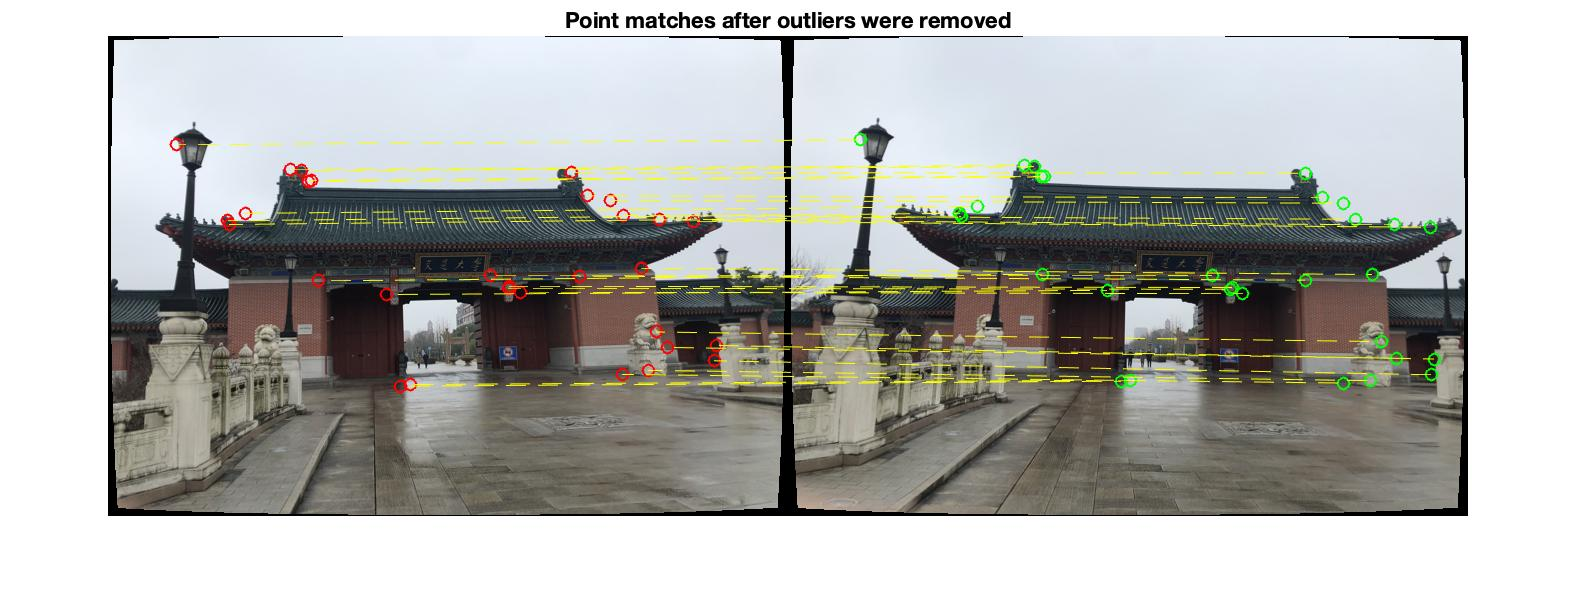
\includegraphics[width=0.9\textwidth]{figures/2.jpg}
\end{center}

发现对应点变少了,但是对应关系依旧是非常的好。
再看一下点云图
\begin{center}
    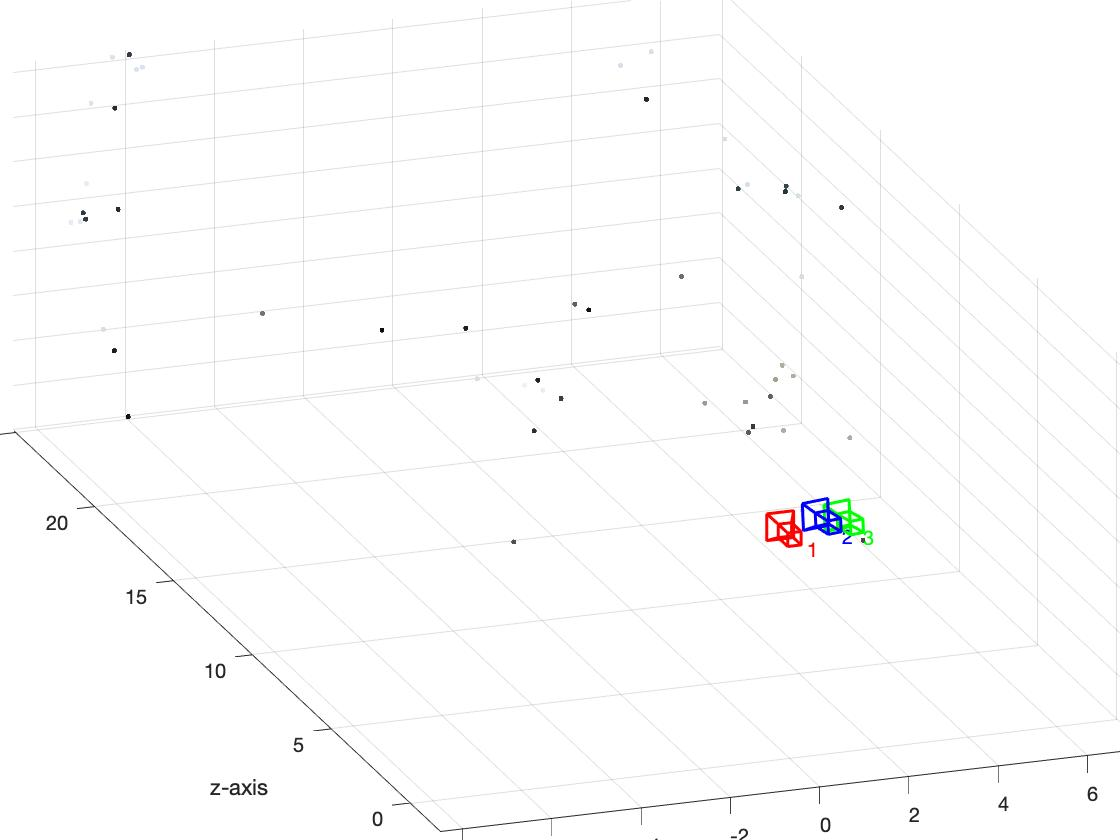
\includegraphics[width=0.9\textwidth]{figures/3.jpg}
\end{center}
可以看到,将特征点与相机位置放到三维坐标系下,可以定性地看出拍照时的实际站位关系,三个相机位置基本正确,特征点的位置也是相对正确的。

最后在看一下经过了bundle Adjustment之后的结果图
\begin{center}
    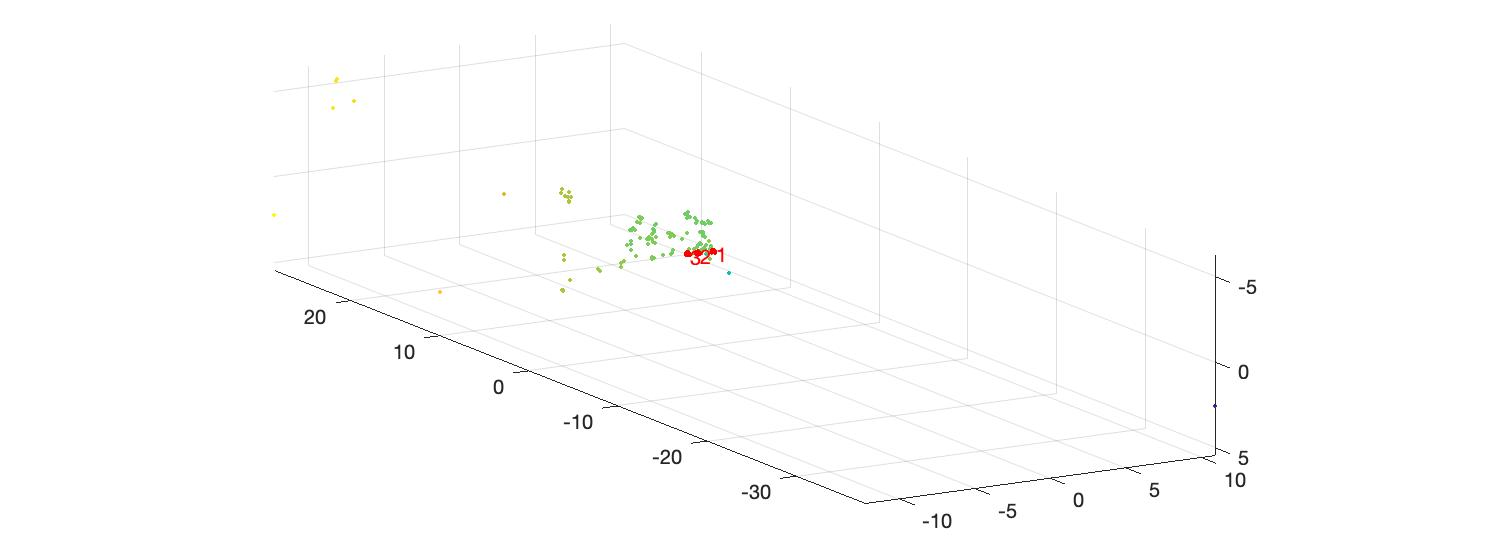
\includegraphics[width=0.9\textwidth]{figures/bundleadjustment.jpg}
\end{center}
可以看出,经过了Bunble Adjutment之后,点云图片相对于之前的图有了一些改变,这也是重投影误差减小的一种体现。



\section{量化分析}
在此使用另外一种方法计算第三个相机视角。就是直接使用第一张图和第三张图进行匹配,求出相对位置关系。

原来的结果和使用直接匹配的方法求出来的结果分别为:
\begin{center}
    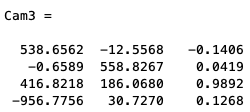
\includegraphics[width=0.4\textwidth]{figures/test1.png}
    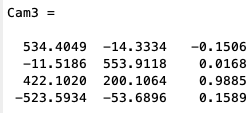
\includegraphics[width=0.4\textwidth]{figures/test2.png}
\end{center}
可以发现,基本上除了少许的一两个值变化比较大,其他的值几乎是没有什么变化,这个不同是由于在匹配的时候原来的方法使用的是已经经过匹配的特征点进行匹配的,精度会比直接匹配来的精确,这也是造成这个差别的原因。

